\documentclass[twocolumn,final]{elsarticle}
%%


%% Stylefile to load MEDIMA template
\usepackage{medima}
\usepackage{framed,multirow}

%% The amssymb package provides various useful mathematical symbols
\usepackage{amssymb}
\usepackage{amsmath}
\usepackage{physics}
\usepackage{booktabs}
\usepackage[ruled,vlined]{algorithm2e}
% Following three lines are needed for this document.
% If you are not loading colors or url, then these are
% not required.
\usepackage{url}
%\usepackage{xcolor}
\usepackage{latexsym}
\usepackage{soul}
\usepackage{xspace}
\usepackage{subcaption}
\usepackage{hyperref}

\usepackage[capitalize]{cleveref}
\crefname{section}{Sec.}{Secs.}
\Crefname{section}{Section}{Sections}
\Crefname{table}{Table}{Tables}
\crefname{table}{Tab.}{Tabs.}
\definecolor{newcolor}{rgb}{.8,.349,.1}

\journal{Medical Image Analysis}

%%%% Custom Imports
% \definecolor{todocolor}{RGB}{200,120,120}
% \sethlcolor{todocolor}
% \newcommand{\todo}[1]{\textcolor{black}{\hl{#1}}}

\def\etal{{et.~al}}
\def\myarch{RadFormer\xspace}

\newcommand{\ra}{\textcolor{Periwinkle}{R1}}
\newcommand{\rb}{\textcolor{PineGreen}{R2}}
\newcommand{\rc}{\textcolor{YellowGreen}{R3}}

\newcommand{\myfirstpara}[1]{\noindent \textbf{#1:}}
%\newcommand{\mypara}[1]{\vspace{0.1em} \myfirstpara{#1}}
\newcommand{\mypara}[1]{\noindent \textit{\textbf{#1:}}}

%\newcommand{\rev}[1]{#1}

\newcommand{\rev}[1]{\textcolor{blue}{#1}}


\newcommand\oast{\stackMath\mathbin{\stackinset{c}{0ex}{c}{0ex}{\ast}{\bigcirc}}}

\newcommand{\beginsupplement}{%
    \setcounter{table}{0}
    \renewcommand{\thetable}{S\arabic{table}}%
    \setcounter{figure}{0}
    \renewcommand{\thefigure}{S\arabic{figure}}%
 }

\begin{document}

\verso{Soumen Basu \textit{et~al.}}

\title{Supplementaty Material \\ \myarch: Transformers with Global-Local Attention for Interpretable and Accurate Gallbladder Cancer Detection}

%\title{Type the title of your paper, only capitalize first
%word and proper nouns\tnoteref{tnote1}}%
%\tnotetext[tnote1]{This is an example for title footnote coding.}

\author[1]{Soumen \snm{Basu}\corref{cor1}}
\cortext[cor1]{Corresponding author.}
\ead{soumen.basu@cse.iitd.ac.in}
\author[1]{Mayank \snm{Gupta}}
\author[2]{Pratyaksha \snm{Rana}}
\author[2]{Pankaj \snm{Gupta}}
\author[1]{Chetan \snm{Arora}}


\address[1]{Department of Computer Science, Indian Institute of Technology Delhi, New Delhi, India}
\address[2]{Department of Radiodiagnosis and Imaging, Postgraduate Institute of Medical Education \& Research, Chandigarh, India}

\maketitle

\section*{Supplementary Material}

\appendix
\beginsupplement

\section{Effect of using other backbones}
%
\begin{table}[t]
   \centering
	\begin{tabular}{lccc}
		\toprule
		\textbf{Backbone} & \textbf{Accuracy} 
		&  \textbf{Specificity} & \textbf{Sensitivity}  \\
		\midrule
		ResNet18 & 0.885$\pm$0.049 & 0.964$\pm$0.042 & 0.908$\pm$0.078 \\
		ResNet34 & 0.883$\pm$0.034 & 0.950$\pm$0.038 & 0.903$\pm$0.084 \\
		ResNet50 & 0.921$\pm$0.062 & 0.961$\pm$0.049 & 0.923$\pm$0.062 \\
		\bottomrule
	\end{tabular}
	\caption{Effect of the choice of global branch backbone on \myarch performance. The local branch is Bagnets-33 for all three cases.}
    \label{tab:ablation-backbone}
\end{table}
We have experimented with different variants of ResNet backbones for the global branch in the \myarch architecture. The performances are reported in \cref{tab:ablation-backbone}. \myarch with ResNet50 global backbone obtains the highest accuracy and sensitivity, while \myarch with ResNet18 backbone obtains the highest specificity.

\section{Attention score visualization in transformer}
%
\begin{figure}
    \centering
    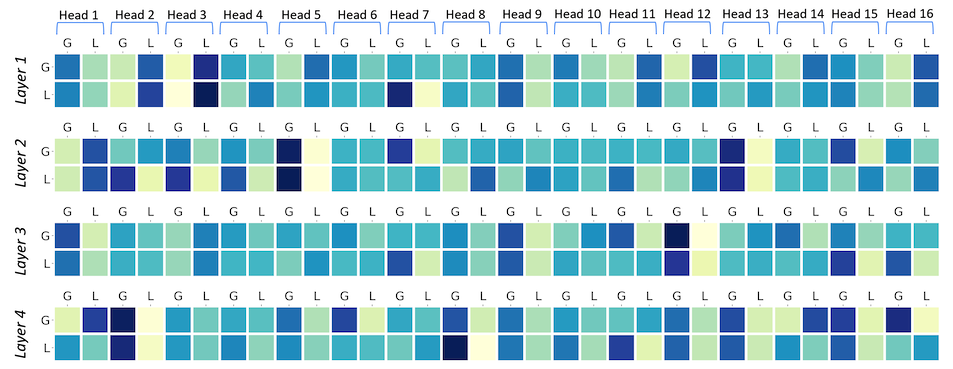
\includegraphics[width=\linewidth]{figs/trans_attn.png}
    \caption{Heatmap of the attention scores of global and local tokens in different transformer layers across all 16 attention heads. The scores are averaged over malignant samples. Low scores are represented with lighter and high scores are represented with darker shades.}
    \label{fig:attn_score}
\end{figure}

\cref{fig:attn_score} shows the visualization of pooled attention scores in different attention heads across the layers. It can be seen that both the global and local tokens influence each other by putting attention to self and the other token. This is an indicator that the attention mechanism is efficiently fusing the global and local features.

\section{Class-wise performance of models}
%
\begin{table}[h]
   \centering
	%\setlength{\tabcolsep}{10pt}
	\resizebox{ \linewidth}{!}{%
	\begin{tabular}{lcccc}
		\toprule
		\multirow{2}{*}{\textbf{Method}} & \multicolumn{4}{c}{\textbf{Accuracy}} \\
		&  \textbf{Overall} & \textbf{Nml.} & \textbf{Ben.} & \textbf{Malg.} \\
		\midrule
		ResNet50 & 0.811$\pm$0.031 & 0.904$\pm$0.040 & 0.812$\pm$0.051 & 0.672$\pm$0.147 \\
		Faster-RCNN & 0.757$\pm$0.053 & 0.720$\pm$0.046 & 0.767$\pm$0.061 & 0.808$\pm$0.104 \\
		ViT & 0.803$\pm$0.078 & 0.764$\pm$0.081 & 0.786$\pm$0.147 & 0.860$\pm$0.068 \\
		GFNet & 0.835$\pm$0.054 & 0.882$\pm$0.053 & 0.829$\pm$0.083 & 0.793$\pm$0.103 \\
		SRC-MT & 0.825$\pm$0.035 & 0.944$\pm$0.040 & 0.764$\pm$0.061 & 0.776$\pm$0.105 \\
		LibAUC & 0.815$\pm$0.028 & 0.886$\pm$0.067 & 0.813$\pm$0.070 & 0.701$\pm$0.152 \\
		GBCNet & 0.921$\pm$0.029 & 0.902$\pm$0.085 & 0.920$\pm$0.052 & 0.919$\pm$0.063 \\
		\midrule
		RadFormer & 0.921$\pm$0.062 & 0.949$\pm$0.069 & 0.906$\pm$0.086 & 0.923$\pm$0.062\\
		\bottomrule
	\end{tabular}
	}
    \caption{Class-wise performance of different models. We report the per-class accuracy for normal, benign, and malignant gallbladders.}
    \label{tab:classwise}
\end{table}

We have also reported the class-wise performance of \myarch and some selected baselines in \cref{tab:classwise}. \myarch works well across different classes. 

\section{Features unmatched to lexicons}
%
There are a total of 65 features in the set of top-10 activated features for each of the malignant samples. Our algorithm matched 32 of the top activated features to radiologist approved lexicons identified in GB-RADS. That is, about 50\% of the set of top-10 malignant features are explainable with our algorithm. However, although there are about 33 features that are unmatched to radiological lexicons, we observed only one of them (id 1607) has been activated for 78\% malignant samples. There are 5 other unmatched features (ids: 283, 481, 683, 973, 1108) that were among the top-10 activated features for 25--35\% of malignant samples. \cref{fig:unknown-new} shows the visualization of these five features. Out of the remaining features, 19 have been activated for less than 10\% and 8 have been activated for 10--25\% malignant samples.

\begin{figure}
    \centering
    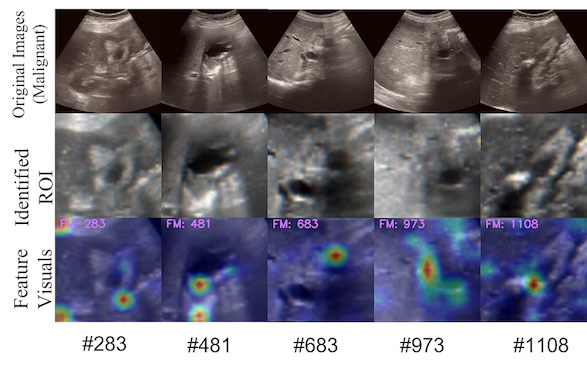
\includegraphics[width=\linewidth]{figs/all-unmatched.png}
    \caption{Visuals of a few top-actived features from the malignant samples that were not matched to any radiological lexicon by our algorithm.}
    \label{fig:unknown-new}
\end{figure}

\end{document}